% la-05-leastsqu.tex

\documentclass[xcolor=dvipsnames]{beamer}
\usepackage{teachbeamer}

\title{Vectors}
\subtitle{{\CourseNumber}, BCIT}

\author{\CourseName}

\date{October 8, 2018}

\begin{document}

\begin{frame}
  \titlepage
\end{frame}

\begin{frame}
  \frametitle{Projection}
  The \alert{projection} $u_{H}$ of a vector $u$ onto a hyperplane $H$
  is the vector in the hyperplane that is ``most similar'' to $u$. The
  formal definition for $u_{H}$ requires that
  \begin{enumerate}
  \item $u$ is in $H$
  \item $(u-u_{H})$ is orthogonal to all basis vectors of $H$
  \end{enumerate}
\end{frame}

\begin{frame}
  \frametitle{Projection}
  \beispiel{Finding a Projection} Let $H$ be the line spanned by
  $\vec{v}=(-1,1)^{\intercal}$ in $\mathbb{R}^{2}$. What is the
  projection $\vec{w}$ of $\vec{u}=(3,-2)^{\intercal}$?
    \begin{figure}[h]
    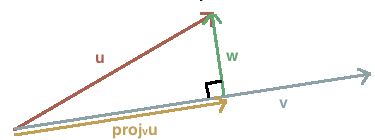
\includegraphics[scale=0.32]{./diagrams/project.png}
  \end{figure}
  Let $\vec{w}=(w_{1},w_{2})^{\intercal}$. Then (1) $\vec{u}-\vec{w}$
  is orthogonal to $\vec{v}$ and (2) $\vec{w}=\alpha\vec{v}$ for some
  $\alpha\in\mathbb{R}$.
  \begin{equation}
    \label{eq:vorahcat}
    \begin{array}{ccccc}
      w_{1}&-&w_{2}&=&5 \\
      w_{1}&+&w_{2}&=&0 \\
    \end{array}
  \end{equation}
Cramer's rule tells us that $\vec{w}=(2.5,-2.5)^{\intercal}$. 
\end{frame}

\begin{frame}
  \frametitle{Projection}
  Let $u=(u_{1},{\ldots},u_{n})^{\intercal}$ be a vector and $H$ be a
  $k$-dimensional hyperplane in the vector space $\mathbb{R}^{n}$. Let
  $x_{1},{\ldots},x_{k}$ be a basis for $H$. Then it is true for all
  vectors $v$ in the hyperplane that
  \begin{equation}
    \label{eq:ahdoogoh}
    \Vert{}u-v\Vert\geq\Vert{}u-u_{H}\Vert
  \end{equation}
  Proof: use the theorem of Pythagoras for
  \begin{equation}
    \label{eq:yoochaev}
    \Vert{}u-v\Vert^{2}=\Vert{}u-u_{H}\Vert^{2}+\Vert{}u_{H}-v\Vert^{2}\geq\Vert{}u-u_{H}\Vert^{2}
  \end{equation}
The claim follows. It illustrates what I mean when I say that $u_{H}$
is the vector in $H$ that is most similar to $u$. 
\end{frame}

\begin{frame}
  \frametitle{Projection}
  \beispiel{Finding Another Projection} What is the projection of
  $\vec{u}=(5,2,10)^{\intercal}$ onto the plane $T$ characterized by
  $2x+y+3z=0$?

  \medskip

  First we find two linearly independent vectors in $H$ to form a
  basis of $H$, for example $\vec{v_{1}}=(1,1,-1)^{\intercal}$ and
  $\vec{v_{2}}=(0,-3,1)^{\intercal}$. The conditions
  \begin{enumerate}
  \item $u_{H}\in{}T$
  \item $(u-u_{H})\perp{}v_{1}$
  \item $(u-u_{H})\perp{}v_{2}$
  \end{enumerate}
  give us the system of linear equations
  \begin{equation}
    \label{eq:faishiso}
    \left[
      \begin{array}{ccc}
        2 & 1 & 3 \\
        -1 & 1 & 1 \\
        0 & 3 & -1
      \end{array}\right]\cdot\left[
      \begin{array}{c}
        \hat{x} \\
        \hat{y} \\
        \hat{z}
      \end{array}\right]=\left[
      \begin{array}{c}
        0 \\
        3 \\
        -4
      \end{array}\right]
  \end{equation}
for which the solution is $u_{H}=(\hat{x},\hat{y},\hat{z})^{\intercal}=(-1,-1,1)^{\intercal}$.
\end{frame}

\begin{frame}
  \frametitle{End of Lesson}
Next Lesson: TBA
\end{frame}

\end{document}

